\documentclass[a4paper,german,12pt,smallheadings]{scrartcl}
\usepackage[T1]{fontenc}
\usepackage[utf8]{inputenc}
\usepackage{babel}
\usepackage{tikz}
\usepackage{geometry}
\usepackage{amsmath}
\usepackage{amssymb}
\usepackage{float}
\usepackage[thinspace,thinqspace,squaren,textstyle]{SIunits}
\restylefloat{table}
\geometry{a4paper, top=15mm, left=20mm, right=40mm, bottom=20mm, headsep=10mm, footskip=12mm}
\linespread{1.5}
\setlength\parindent{0pt}
\begin{document}
\begin{center}
\bfseries % Fettdruck einschalten
\sffamily % Serifenlose Schrift
\vspace{-40pt}
Analytische Mechanik, Sommersemester 2013, 4. Blatt \\
Luis Herrmann und Markus Fenske, Tutor: Clemens Meyer zu Rheda
\vspace{-10pt}
\end{center}
\section*{Aufgabe 1}

In der Zeichnung ist eine Rotation um die x-Achse dargestellt (z-Achse nicht sichtbar), in der Aufgabe rechnen wir jedoch wie gefragt den Fall einer Rotation um die y-Achse durch.

%\resizebox{10cm}{10cm}{%
\begin{figure}[H]
  \begin{center}
    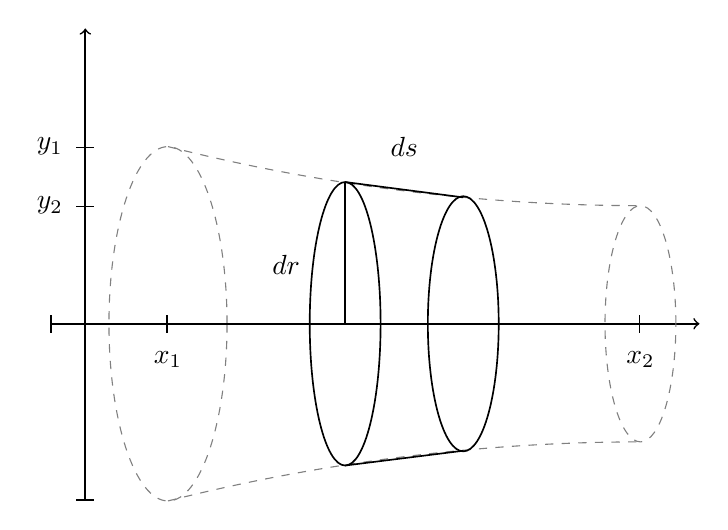
\begin{tikzpicture}[scale=1.5]
      \draw[dashed,color=gray] (0,1.5) ellipse (0.5 and 1.5);% right half of the left ellipse
      \draw[dashed,color=gray] (0,0) parabola bend (4,0.5) (4,0.5);% bottom line
      \draw[dashed,color=gray] (0,3) parabola bend (4,2.5) (4,2.5);% top line
      \draw[semithick] (1.5,1.5) ellipse (0.3 and 1.2);% left du
      \draw[-,semithick] (1.5,2.7) -- (2.5,2.57);
      \draw[-,semithick] (1.5,1.5) -- (1.5,2.7); % dr
      \draw (1.0,2) node {$dr$};
      \draw (2.0,3) node {$ds$};
      \draw[semithick] (2.5,1.5) ellipse (0.3 and 1.08);% left du
      \draw[-,semithick] (1.5,0.3) -- (2.5,0.425); % bottom ds
      \draw[|-|,semithick] (-1,1.5) -- (0,1.5);
      \draw[-|,semithick] (0,1.5) -- (4,1.5);
      \draw[->,semithick] (4,1.5) -- (4.5,1.5);
      \draw[|-|,semithick] (-0.7,0) -- (-0.7,2.5);
      \draw[-|,semithick] (-0.7,2.5) -- (-0.7,3);
      \draw[->,semithick] (-0.7,3) -- (-0.7,4);
      \draw (-1,2.5) node {$y_2$};
      \draw (-1,3) node {$y_1$};
      \draw[dashed,color=gray] (4,1.5) ellipse (0.3 and 1);% right ellipse
      \draw (0,1.2) node {$x_1$};
      \draw (4,1.2) node {$x_2$};
    \end{tikzpicture}
  \end{center}
  \caption{Rotationskörper mit Radiuselement $dr$ und Linienelement $ds$}
\end{figure}
%}

Der Abstand zwischen den Punkten P1 und P2 über die Kurve beträgt:
\begin{equation}
S=\int\limits_S\ ds
\end{equation}
Dabei ist das Wegelement $ds$:
\begin{equation}
ds=\sqrt{dx^2+dy^2}=dx\sqrt{1+\dot{y}^2} \quad mit \quad \dot{y}=\frac{\partial y}{\partial x}
\end{equation}
Für die Rotationsoberfläche gilt:
\begin{equation}
O=\int\limits_O dO \quad \text{wobei} \quad dO=2\pi x ds
\end{equation}
Unter Verwendung vom zuvor gefundenen Ausdruck für ds (3) erhalten wir:
\begin{equation}
O=\int\limits_{x_1}^{x_2} 2\pi x \sqrt{1+\dot{y}^2} \; dx = O=2\pi \int\limits_{x_1}^{x_2} x \sqrt{1+\dot{y}^2} \; dx
\end{equation}
Wobei O extremal, genauer gesagt minimal werden soll. Dieses Problem ist äquivalent zu einer Formulierung über die Euler-Lagrange-Gleichung:
\begin{equation}
\frac{d}{dx}\left(\frac{\partial \mathcal{F}}{\partial \dot{y}}\right)-\frac{\partial \mathcal{F}}{\partial y}=0 \quad mit \quad \mathcal{F}(x,y,\dot{y})
\end{equation}
In diesem Fall ist:
\begin{equation}
\mathcal{F}=x \sqrt{1+\dot{y}^2}
\end{equation}
Wir bilden also:
\begin{equation}
\frac{\partial \mathcal{F}}{\partial y}=\frac{\partial x \sqrt{1+\dot{y}^2}}{\partial y}=0
\end{equation}
Da weder $x$ noch $\dot{y}$ explizit von $y$ abhängen.
\begin{equation}
\frac{\partial \mathcal{F}}{\partial \dot{y}}=\frac{\partial x \sqrt{1+ \dot{y}^2}}{\partial \dot{y}}=0 + \frac{2x \dot{y}}{2 \sqrt{1+ \dot{y}^2}}=\frac{x \dot{y}}{\sqrt{1+ \dot{y}^2}}
\end{equation}
Setzen wir (7) und (8) in (5) ein, so erhalten wir:
\begin{align*}
\frac{d}{dx}\left(\frac{x \dot{y}}{\sqrt{1+ \dot{y}^2}}\right)-\frac{\partial x \sqrt{1+\dot{y}^2}}{\partial y}=0\\
\Leftrightarrow \frac{d}{dx}\left(\frac{x \dot{y}}{\sqrt{1+ \dot{y}^2}}\right)-0=0
\end{align*}
Und daraus folgt, dass:
\begin{equation}
\frac{x \dot{y}}{\sqrt{1+ \dot{y}^2}}=const.
\end{equation}
Nennen wir diese Konstante $A$ und formen nach $\dot{y}$ um:
\begin{align*}
\frac{x \dot{y}}{\sqrt{1+ \dot{y}^2}}=A\\
\Leftrightarrow x \dot{y}=A \sqrt{1+\dot{y}^2}\\
\Leftrightarrow x^2 \dot{y}^2=A^2\left(1+\dot{y}^2\right)\\
\Leftrightarrow x^2=A^2 \frac{1+\dot{y}^2}{\dot{y}^2}\\
\Leftrightarrow \frac{x^2}{A^2}=\frac{1}{\dot{y}^2}+1\\
\Leftrightarrow \frac{x^2}{A^2}-1=\frac{1}{\dot{y}^2}\\
\Leftrightarrow \dot{y}^2=\frac{1}{\left(\frac{x^2}{A^2}-1\right)}\\
\Leftrightarrow \dot{y}^2=\frac{A^2}{\left(x^2-A^2\right)}\\
\Leftrightarrow \dot{y}=\frac{A}{\sqrt{x^2-A^2}}
\end{align*}
Damit ist es ein leichtes, die Kurve $y$ auszurechnen:
\begin{equation}
y=\int \dot{y} \; dx=\int \frac{A}{\sqrt{x^2-A^2}} \; dx=A \int \frac{1}{\sqrt{x^2-A^2}} \; dx
\end{equation}
Durch Nachschlagen in der Integraltabelle findet man, dass:
\begin{equation}
\int \frac{1}{\sqrt{x^2-a^2}} \; dx=A \sinh\left(\frac{x}{a}\right)
\end{equation}
Und in:
\begin{equation}
y=A \sinh\left(\frac{x}{A}\right) \quad\\ 
\end{equation}
...mit den Bedingungen:
\begin{equation}
\quad y_1=\sinh\left(\frac{x_1}{A}\right) \quad und \quad y_2=\sinh\left(\frac{x_2}{A}\right)
\end{equation}

\section*{Aufgabe 2}
\subsection*{Teilaufgabe 1}
Aufstellen der Lagrange-Funktion:
\begin{equation}
V=mgy=mg\left(at+bt^2\right)
\end{equation}
\begin{equation}
T=\frac{m}{2} \dot{y}^2
\end{equation}
Wobei wir den Ansatz verwenden:
\begin{equation}
y=at+bt^2 \Rightarrow \dot{y}=a+2bt \Rightarrow \dot{y}^2=a^2+4abt+4b^2t^2
\end{equation}
Und wir erhalten:
\begin{equation}
\mathcal{L}=T-V=\frac{m}{2} \left(a^2+4abt+4b^2t^2\right) - mg\left(at+bt^2\right)
\end{equation}
\subsection*{Teilaufgabe 2}
Gesucht ist das Ergebnis des Wirkungsintegrals:
\begin{equation}
S=\int\limits_{t_0}^{0} \mathcal{L} \; dt
\end{equation}
Einsetzen der Gleichung aus Teilaufgabe 1 und ausrechnen:
\begin{align*}
S=\int\limits_{0}^{t_0} \frac{m}{2} \left(a^2+4abt+4b^2t^2\right) - mg\left(at+bt^2\right)\\
\Leftrightarrow S=\frac{m}{2} \left(a^2t_0+\frac{4}{3}b^2t_0^3+2abt_0^2\right)-mg\left(\frac{1}{2} at_0^2+ \frac{1}{3} bt_0^3\right)
\end{align*}
\subsection*{Teilaufgabe 3}
Zur Minimierung des Wirkungsintegrals in Abhängigkeit von $a$ und $b$ bilden wir die partiellen Ableitungen nach $a$ und $b$:
\begin{equation}
\frac{\partial S}{\partial a}=\frac{\partial \frac{m}{2} \left(a^2t_0+\frac{4}{3}b^2t_0^3+2abt_0^2\right)-mg\left(\frac{1}{2} at_0^2+ \frac{1}{3} bt_0^3\right)}{\partial a}=\frac{m}{2}\left(2at_0+2bt_0^2\right)-\frac{mgt_0^2}{2}\overset{!}{=}0
\end{equation}
\\
\begin{equation}
\frac{\partial S}{\partial b}=\frac{\partial \frac{m}{2} \left(a^2t_0+\frac{4}{3}b^2t_0^3+2abt_0^2\right)-mg\left(\frac{1}{2} at_0^2+ \frac{1}{3} bt_0^3\right)}{\partial b}=\frac{m}{2}\left(\frac{8}{3}bt_0^3+2at_0^2\right)-\frac{mgt_0^3}{3}\overset{!}{=}0
\end{equation}
Gesucht ist die Lösung des linearen Gleichungssystems:
\begin{align*}
a+bt_0-\frac{gt_0}{2}=0\\
\frac{4}{3}bt_0+a-\frac{gt_0}{3}=0\\
\\
\Leftrightarrow a=\frac{gt_0}{2}-bt_0\\
\Leftrightarrow \frac{4}{3}bt_0+\frac{gt_0}{2}-bt_0-\frac{gt_0}{3}=0\\
\\
\Leftrightarrow a=\frac{gt_0}{2}-bt_0\\
\Leftrightarrow \frac{1}{3}bt_0+\frac{1}{6}gt=0\\
\\
\Leftrightarrow a=\frac{gt_0}{2}--\frac{1}{2}gt_0=0\\
\Leftrightarrow b=-\frac{1}{2}g\\
\\
\end{align*}
Und erhalten somit, dass das Wirkungsintegral extremal wird für:
\begin{equation}
y=-\frac{gt^2}{2}
\end{equation}
Wir prüfen, ob es maximal oder minimal wird:
\begin{align*}
\frac{\partial^2 S}{\partial a^2}=\frac{\partial \frac{m}{2}\left(2at_0+2bt_0^2\right)-\frac{mgt_0^2}{2}}{\partial a}=\frac{m}{2}\left(2t_0\right)=mt_0=m \sqrt{\frac{2y_0}{g}}>0
\end{align*}
...da wir $y_0$ und $g$ als positiv definieren.
\begin{align*}
\frac{\partial^2 S}{\partial b^2}=\frac{\partial \frac{m}{2}\left(\frac{8}{3}bt_0^3+2at_0^2\right)-\frac{mgt_0^3}{3}}{\partial b}=\frac{m}{2}\left(\frac{8}{3}t_0^3\right)=\frac{4m}{3} \left(\frac{2y_0}{g}\right)^{3/2}>0
\end{align*}
...siehe oben. Tatsächlich wird das Wirkungsintegral also minimal für:
\begin{equation}
y=-\frac{gt^2}{2}
\end{equation}
\\
\section*{Aufgabe 3}
\subsection*{Vorspann}
Auf dem letzten Zettel hatten wir Folgendes gezeigt:

Für den Klotz wählen wir die Koordinaten $(x_1, y_1)$, für den Keil die
Koordinaten $(x_2, y_2)$, jeweils vom Ursprung aus.

Der Keil bewegt sich nur auf seiner Unterlage. Der Klotz hingegen nur auf der
Schräge des Keils. Dies führt zu den folgenden Zwangsbedingungen:


\begin{align*}
  y_1 &= (x1-x2) \tan \alpha \\
  y_2 &= 0
\end{align*}

Sei $T_1$ die kinetische Energie des Klotzes und $T_2$ die des Keils. Die Masse
des Klotzes sei $m_1$, die Masse des Keils sei $m_2$.

\begin{align*}
  T_1 &= \frac{1}{2} m_1 \left(\dot{x_1}^2 + \dot{y_1}^2\right) \\
  T_2 &= \frac{1}{2} m_2 \dot{x_2}^2
\end{align*}

Durch Einsetzen der Zwangsbedingungen erhalten wir:

\begin{align*}
  T_1 &= \frac{1}{2}m_1\dot{x_1}^2 + \frac{1}{2}m_2 (\dot{x_1}^2 - 2\dot{x_1}\dot{x_2}+\dot{x_2}^2) \tan^2 \alpha \\
  T_2 &= \frac{1}{2} m_2 \dot{x_2}^2
\end{align*}

Für die kinetische Energie insgesamt dann also:

\begin{align*}
  T = \frac{1}{2}m_1\dot{x_1}^2 + \frac{1}{2}m_2 (\dot{x_1}^2 - 2\dot{x_1}\dot{x_2}+\dot{x_2}^2) \tan^2 \alpha + \frac{1}{2} m_2 \dot{x_2}^2
\end{align*}

Eine potentielle Energie erhält nur der Klotz, denn der Keil ändert seine Höhe nicht. Somit ist:

\begin{align*}
  V = V_2 = m_2gy_2 = m_2g (x_1 - x_2) \tan \alpha
\end{align*}

Damit ist die Lagrangefunktion insgesamt:

\begin{align*}
  \mathcal{L} = T -V = \frac{1}{2}m_1\dot{x_1}^2 + \frac{1}{2} m_2 (\dot{x_1}^2 - 2\dot{x_1}\dot{x_2}+\dot{x_2}^2) \tan^2 \alpha + \frac{1}{2} m_2 \dot{x_2}^2 - m_2g (x_1 - x_2) \tan \alpha
\end{align*}

Die Bewegungsgleichungen ergeben sich durch Anwendung der Euler-Lagrange-Gleichung:

\begin{align*}
  \left(\frac{d}{dt}\frac{\partial \mathcal{L}}{\partial \dot{q_i}} - \frac{\partial \mathcal{L}}{\partial q_i}\right)= 0
\end{align*}

Für die $x_1$-Koordinate:

\begin{align*}
  \frac{\partial \mathcal{L}}{\partial x_1} &= -mg \tan \alpha \\
  \frac{d}{dt}\frac{\partial \mathcal{L}}{\partial \dot{x_1}} &= \frac{d}{dt} m_1 \dot{x_1} + m_2\dot{x_1}\tan^2 \alpha - m_2\dot{x_2} \tan^2 \alpha \\
                                                  &= m_1\ddot{x_1} + m_2 \ddot{x_1} \tan^2 \alpha - m_2 \ddot{x_2} \tan^2 \alpha \\
  \Rightarrow\quad &m_1\ddot{x_1} + m_2 \ddot{x_1} \tan^2 \alpha - m_2 \ddot{x_2} \tan^2 \alpha = -mg \tan \alpha
\end{align*}

Für $x_2$ ergibt sich:

\begin{align*}
  \frac{\partial \mathcal{L}}{\partial x_2} &= mg \tan \alpha \\
  \frac{d}{dt}\frac{\partial \mathcal{L}}{\partial \dot{x_2}} &= \frac{d}{dt} m_2\dot{x_2} \tan^2 \alpha - m_2 \dot{x_1} \tan^2 \alpha + m_2\dot{x_2} \\
  &= \ddot{x_2}(m_2+m_2 \tan^2 \alpha) - \ddot{x_1} m_2 \tan^2 \alpha \\
  \Rightarrow\quad &\ddot{x_2}(m_2+m_2 \tan^2 \alpha) - \ddot{x_1} m_2 \tan^2 \alpha = mg \tan \alpha
\end{align*}

Um zu zeigen, dass beide Massen konstant beschleunigt werden, addieren wir die beiden Bewegungsgleichungen:

\begin{align*}
&\ddot{x_1}(m_1+m_2 \tan^2 \alpha -m_2 \tan^2 \alpha)+\ddot{x_2}(m_2+m_2 \tan^2 \alpha - m_2 \tan^2 \alpha)=mg \tan \alpha - mg \tan \alpha \\
\Leftrightarrow\quad & \ddot{x_1} m_1 = -\ddot{x_2} m_2
\end{align*}

% iblue: Habe das hinzugefügt.
Setzt man dies in die zweite Bewegungsgleichung ein, erhält man:

\begin{align*}
  &\ddot{x_2}(m_2+m_2 \tan^2 \alpha) + \ddot{x_2} \frac{m_2^2}{m_1} \tan^2 \alpha = mg \tan \alpha \\
  \Leftrightarrow \quad &\ddot{x_2} (m_2+m_2 \tan^2 \alpha + \frac{m_2^2}{m_1} \tan^2 \alpha) = mg \tan \alpha \\
  \Leftrightarrow \quad &\ddot{x_2} = \frac{mg \tan \alpha}{m_2+m_2 \tan^2 \alpha + \frac{m_2^2}{m_1} \tan^2 \alpha}
\end{align*}

\subsection*{Teilaufgabe 1}
Die Zwangsbedingungen lauten:
\begin{align*}
\tan\alpha=\frac{y_2}{x_1-x_2} \quad \Leftrightarrow \quad y_2=\tan\alpha \left(x_1-x_2\right) \quad \Rightarrow \quad f_1=y_2-\tan\alpha \left(x_1-x_2\right)=0\\
f_2=y_1=0
\end{align*}
Aufstellen der Lagrange-Funktion:
\begin{align*}
T_1=\frac{m_1}{2} \left(\dot{x_1}^2+\dot{y_1}^2\right)\\
T_2=\frac{m_2}{2} \left(\dot{x_2}^2+\dot{y_2}^2\right)\\
V_1=m_1gy_1\\
V_2=m_2gy_2\\
\Rightarrow \mathcal{L}=\frac{m_1}{2} \left(\dot{x_1}^2+\dot{y_1}^2\right)+\frac{m_2}{2} \left(\dot{x_2}^2+\dot{y_2}^2\right)-m_1gy_1-m_2gy_2
\end{align*}
Für die Zwangskräfte gilt:
\begin{equation}
\frac{d}{dt}\left(\frac{\partial \mathcal{L}}{\partial \dot{q_i}}\right)-\frac{\partial \mathcal{L}}{\partial q_i}=\sum\limits_j \lambda_j \frac{\partial f_j}{\partial q_i}
\end{equation}
Für $x_1$, $x_2$, $y_1$ und $y_2$:
\begin{align}
x_1: & \quad \frac{d}{dt} \left(m_1 \dot{x_1}\right)=-\lambda_1 \tan \alpha \quad \Rightarrow \quad m_1 \ddot{x_1}=-\lambda_1 \tan \alpha\\
x_2: & \quad  \frac{d}{dt} \left(m_2 \dot{x_2}\right)=\lambda_1 \tan \alpha \quad \Rightarrow \quad m_2 \ddot{x_2}=\lambda_1 \tan \alpha\\
y_1: & \quad \frac{d}{dt} \left(m_1 \dot{y_1}\right)+m_1g=\lambda_2 \quad \Rightarrow \quad m_1 \ddot{y_1}+m_1g=\lambda_2\\
y_2: & \quad \frac{d}{dt} \left(m_2 \dot{y_2}\right)+m_2g=\lambda_1 \quad \Rightarrow \quad m_2 \ddot{y_2}+m_2g=\lambda_1
\end{align}
Wir verwenden nun:
\begin{align*}
y_1=0 \quad \Rightarrow \quad \ddot{y_1}=0
y_2=\tan \alpha \left(x_1-x_2\right) \quad \Rightarrow \quad \ddot{y_2}=\tan \alpha \left(\ddot{x_1}-\ddot{x_2}\right)
\end{align*}
Und erhalten nach Einsetzen:
\begin{align*}
x_1: & \quad m_1 \ddot{x_1}=-\lambda_1 \tan \alpha\\
x_2: & \quad m_2 \ddot{x_2}=\lambda_1 \tan \alpha\\
y_1: & \quad m_1g=\lambda_2\\
y_2: & \quad m_2 \tan \alpha \left(\ddot{x_1}-\ddot{x_2}\right)+m_2g=\lambda_1
\end{align*}
Des weiteren finden wir mit $x_1$ und $x_2$:
\begin{equation}
m_2 \ddot{x_2}=-m_1 \ddot{x_1}
\end{equation}
Einsetzen von $\lambda_1$ in $x_1$ und $x_2$ liefert:
\begin{align*}
x_1: & \quad m_1 \ddot{x_1}=-\left(m_2 \tan \alpha \left(\ddot{x_1}-\ddot{x_2}\right)+m_2g\right) \tan \alpha\\
x_2: & \quad m_2 \ddot{x_2}=\left(m_2 \tan \alpha \left(\ddot{x_1}-\ddot{x_2}\right)+m_2g\right) \tan \alpha\\
\\
\Leftrightarrow x_1: & \quad m_1 \ddot{x_1}=-\left(m_2 \tan \alpha \left(\ddot{x_1}+\frac{\ddot{x_1}m_1}{m_2}\right)+m_2g\right) \tan \alpha\\
\Leftrightarrow x_2: & \quad m_2 \ddot{x_2}=\left(m_2 \tan \alpha \left(\frac{\ddot{-x_2}m_2}{m_1}-\ddot{x_2}\right)+m_2g\right) \tan \alpha\\
\\
\Leftrightarrow x_1: & \quad m_1 \ddot{x_1}=-\left(m_2 \tan \alpha \; \ddot{x_1} \left(1+\frac{m_1}{m_2}\right)+m_2g\right) \tan \alpha\\
\Leftrightarrow x_2: & \quad m_2 \ddot{x_2}=\left(-m_2 \tan \alpha \; \ddot{x_2} \left(\frac{m_2}{m_1}+1\right)+m_2g\right) \tan \alpha\\
\\
\Leftrightarrow x_1: & \quad m_1 \ddot{x_1}=-m_2 \tan^2 \alpha \; \ddot{x_1} \left(1+\frac{m_1}{m_2}\right)-m_2g \tan \alpha\\
\Leftrightarrow x_2: & \quad m_2 \ddot{x_2}=-m_2 \tan^2 \alpha \; \ddot{x_2} \left(\frac{m_2}{m_1}+1\right)+m_2g \tan \alpha\\
\\
\Leftrightarrow x_1: & \quad \ddot{x_1} \left(m_1+m_2 \tan^2 \alpha \left(1+\frac{m_1}{m_2}\right)\right)=-m_2g \tan \alpha\\
\Leftrightarrow x_2: & \quad \ddot{x_2} \left(1+\tan^2 \alpha \left(\frac{m_2}{m_1}+1\right) \right)=g \tan \alpha\\
\\
\Leftrightarrow x_1: & \quad \ddot{x_1}=-\frac{m_2g \tan \alpha}{\left(m_1+m_2 \tan^2 \alpha \left(1+\frac{m_1}{m_2}\right)\right)}\\
\Leftrightarrow x_2: & \quad \ddot{x_2}=\frac{g \tan \alpha}{\left(1+\tan^2 \alpha \left(\frac{m_2}{m_1}+1\right) \right)}\\
\end{align*}
Zuletzt ermitteln wir $\ddot{y_2}$:
\begin{align*}
& \quad \ddot{y_2}=\left(\ddot{x_1}-\ddot{x_2}\right) \tan \alpha\\
\Leftrightarrow & \quad \ddot{y_2}=\left(\ddot{x_1}+\frac{\ddot{x_1}m_1}{m_2}\right) \tan \alpha\\
\Leftrightarrow & \quad \ddot{y_2}=\left(\frac{m_2+m_1}{m_2}\right) \tan \alpha \; \ddot{x_1}\\
\Leftrightarrow & \quad \ddot{y_2}=-\frac{m_2g\tan^2 \alpha}{\left(m_1+m_2\tan^2 \alpha \left(1+\frac{m1}{m2}\right)\right)} \frac{m_2+m_1}{m_2}\\
\Leftrightarrow & \quad \ddot{y_2}=-\frac{\left(m_1+m_2\right)g\tan^2 \alpha}{\left(m_1+m_2\tan^2 \alpha \left(1+\frac{m_1}{m_2}\right)\right)}\\
\end{align*}
Die Zwangskräfte lauten also:
\begin{align*}
& Z_{x_1}=-\lambda_1 \tan \alpha=-\frac{m_1 m_2 g \tan \alpha}{\left(m_1+m_2 \tan^2 \alpha \left(1+\frac{m_1}{m_2}\right)\right)}\\
\\
& Z_{x_2}=\lambda_1 \tan \alpha=\frac{m_2 g \tan \alpha}{\left(1+\tan^2 \alpha \left(\frac{m_2}{m_1}+1\right) \right)}=\frac{m_1 m_2 g \tan \alpha}{\left(m_1+m_2 \tan^2 \alpha \left(1+\frac{m_1}{m_2}\right)\right)}\\
\\
& Z_{y_1}=\lambda_2=m_1g\\
\\
& Z_{y_2}=\lambda_1=m_2\left(-\frac{\left(m_1+m_2\right)g\tan^2 \alpha}{\left(m_1+m_2\tan^2 \alpha \left(1+\frac{m_1}{m_2}\right)\right)}+g\right)
\end{align*}

\section*{Aufgabe 4}
\subsection*{Teilaufgabe 1}
Wir wählen für das Problem Zylinderkoordinaten.\\
\\
Es gibt nur eine Zwangsbedingung. Sie lautet:
\begin{align*}
\frac{r}{z}=\tan \alpha \quad \Rightarrow \quad f_1=r-z \tan \alpha =0
\end{align*}
Aufstellen der Lagrange-Funktion:
\begin{equation}
T=\frac{m}{\dot{r}^2+r^2\dot{\phi}^2+\dot{z}^2}
\end{equation}
\begin{align*}
V=mgz
\end{align*}
\begin{align*}
\mathcal{L}=T-V=\frac{m}{2} \left(\dot{r}^2+r^2\dot{\phi}^2+\dot{z}^2\right) -mgz
\end{align*}

\subsection*{Teilaufgabe 2}
Setze Zwangsbedingungen ein:
\begin{align*}
\mathcal{L}=\frac{m}{2} \left(\dot{r}^2+r^2\dot{\phi}^2+\frac{\dot{r}^2}{\tan^2 \alpha}\right)-\frac{mgr}{\tan \alpha}
\end{align*}
Entwickeln der Lagrange-Gleichung 2.Art:
\begin{align*}
r: & \quad \frac{\partial \mathcal{L}}{\partial r}=mr\dot{\phi}^2-\frac{mg}{\tan \alpha}\\
& \quad \frac{d}{dt}\left(\frac{\partial \mathcal{L}}{\partial \dot{r}}\right)=\frac{d}{dt}\left(m\dot{r}+\frac{m\dot{r}}{\tan^2 \alpha}\right)=m \ddot{r}+\frac{m \ddot{r}}{\tan^2 \alpha}\\
\phi: & \quad \frac{\partial \mathcal{L}}{\partial \phi}=0 \quad \text{da $\mathcal{L}$ nicht explizit von $\phi$ abhängt.}\\
& \quad \frac{d}{dt}\left(\frac{\partial \mathcal{L}}{\partial \dot{\phi}}\right)=\frac{d}{dt}\left(mr^2\dot{\phi}^2\right)\overset{!}{=}0
\end{align*}
Wir erhalten eine inhomogene Differenzialgleichung:
\begin{equation*}
\ddot{r} \left(1+\frac{1}{\tan^2 \alpha}\right)-r\dot{\phi}^2=\frac{g}{\tan \alpha}
\end{equation*}

\subsection*{Teilaufgabe 3}

Für die Zwangskräfte gilt:
\begin{equation*}
\frac{d}{dt}\left(\frac{\partial \mathcal{L}}{\partial \dot{q_i}}\right)-\frac{\partial \mathcal{L}}{\partial q_i}=\sum\limits_j \lambda_j \frac{\partial f_j}{\partial q_i}\\
\end{equation*}
Wir erhalten damit:
\begin{align*}
r: & \quad \frac{d}{dt}\left(m\dot{r}\right)-mr\dot{\phi}^2=\lambda_1 \quad \Leftrightarrow \quad m\ddot{r}-mr\dot{\phi}^2=\lambda_1\\
\phi: & \quad \frac{d}{dt}\left(mr^2\dot{\phi}\right)=0\\
z: & \quad \frac{d}{dt}\left(m\dot{z}\right)+mg=-\lambda_1 \tan \alpha \quad \Leftrightarrow \quad m\ddot{z}+mg=-\lambda_1 \tan \alpha
\end{align*}
Nun benutzen wir:
\begin{equation}
z=\frac{r}{\tan \alpha} \quad \Rightarrow \quad \ddot{z}=\frac{\ddot{r}}{\tan \alpha}
\end{equation}
Und setzen ein in 'z:':
\begin{align*}
& \quad m\left(\frac{\ddot{r}}{\tan \alpha}\right) +mg=-\lambda \tan \alpha\\
\Leftrightarrow & \quad \frac{\ddot{r}}{\tan \alpha}+g=-\frac{\lambda \tan \alpha}{m}\\
\Leftrightarrow & \quad \frac{\ddot{r}}{\tan \alpha}=-\frac{\lambda \tan \alpha}{m}-g\\
\Leftrightarrow & \ddot{r}=-\frac{\lambda \tan^2 \alpha +mg \tan}{m}\\
\end{align*}
Einsetzen des Ergebnisses in 'r:' liefert:\\
\begin{align*}
& \quad m \left(-\frac{\lambda \tan^2 \alpha +mg \tan}{m}\right) -mr \dot{\phi}^2=\lambda\\
\Leftrightarrow & \quad \lambda=-\lambda \tan \alpha -mg \tan \alpha m r \dot{\phi}^2\\
\Leftrightarrow & \quad \lambda\left(1+\tan^2 \alpha\right)=-mg \tan \alpha -mr \dot{\phi}^2\\
\Leftrightarrow & \quad \lambda=-\frac{mg \tan \alpha + mr \dot{\phi}^2}{\left(1+\tan^2 \alpha\right)}\\
\Leftrightarrow & \quad \lambda=-\frac{mg \tan \alpha + mr \dot{\phi}^2}{1\cos^2 \alpha}\\
\Leftrightarrow & \quad \lambda=-m \cos^2 \alpha \left(g \tan \alpha + r \dot{\phi}^2 \right)
\end{align*}

\subsection*{Teilaufgabe 4}
Der absolute Wert der Zwangskraft ist die vektorielle Summe der einzelnen Zwangskräfte:
\begin{equation*}
Z=\sqrt{\sum \limits_j Z_j^2}
\end{equation*}
Einsetzen der Zwangskräfte aus der vorherigen Teilaufgabe liefert:
\begin{align*}
& \quad Z=\sqrt{\lambda^2\left(-\lambda \tan \alpha\right)^2}
\Leftrightarrow & \quad Z=\sqrt{\lambda^2(1+\tan^2 \alpha)}\\
\Leftrightarrow & \quad Z=\sqrt{\frac{\lambda^2}{cos^2 \alpha}}\\
\Leftrightarrow & \quad Z=\frac{\lambda}{\cos \alpha}\\
\end{align*}
Nun setzen wir unser Ergebnis von Teilaufgabe 3 ein:
\begin{align*}
\Leftrightarrow & \quad Z=\frac{-m \cos \alpha \left(g \tan \alpha+r\dot{\phi}^2\right)}{\cos \alpha}\\
\Leftrightarrow & \quad Z=-m \cos \alpha \left(g \tan \alpha+r\dot{\phi}^2\right)\\
\Leftrightarrow & \quad Z=-m \left(g \sin \alpha+r \cos \alpha \; \dot{\phi}^2\right)
\end{align*}

\end{document}